% !TeX spellcheck = es_ES
\chapter{Implementación}
\label{ch:chap04}

El siguiente capítulo desarrolla los detalles de implementación y optimización de los algoritmos para computar los factores de forma simples y extendidos.

\section{Cálculo de factores de forma de la componente difusa}
\label{sec:dif-impl}

Tal como se expresa en la Sección 2.2.2, se implementaron dos algoritmos para el cálculo de factores de forma. El primero está basado en el método del hemi-cubo y el segundo está basado en el trazado de rayos de forma determinista utilizando un hemisferio de Beckes y Beckers \cite{Beckers}.

\subsection{Algoritmo del hemi-cubo}

El algoritmo del hemi-cubo (Sección 2.2.2) fue implementado utilizando la API OpenGL que provee de interfaces de alto nivel para la programación de tarjetas gráficas, facilitando el uso del algoritmo del Z-Buffer y el manejo de memoria en la GPU.

Para implementar el cálculo de factores de forma se implementó la función \verb|computeFormFactors| de la Figura \ref{img:procesado}. Recordando la arquitectura diseñada, la función debe computar completamente la matriz de factores de forma. Esta función sigue las siguientes de etapas:

\begin{enumerate}
	\item En primera instancia, son configurados los \textit{buffers} en memoria necesarios para representar el hemi-cubo.
	Para ello, se crea un \textit{Frame Buffer Object} en la GPU que está compuesto de 5 texturas, cada una de ellas correspondiente a una de las caras a dibujar. Cabe destacar, que estas texturas se componen de dos imágenes: una conteniendo enteros sin signo que son utilizados para representar el \verb|id| de los parches vistos desde el centro del hemi-cubo y la restante contiene los valores de profundidad necesarios para el algoritmo del Z-Buffer.
	\item En la segunda etapa se establecen las matrices de transformación de vista, es decir, las transformaciones que alinean el volúmen de vista al hemi-cubo. Esto implica trasladar el origen de vista hacia el baricentro de la cara en cuestión, y alinearla a su normal.
	\item En la tercera etapa se procede a dibujar cada objeto en la escena desde el parche considerado en las cinco texturas que componen el hemi-cubo. Con el objetivo de tener el mejor rendimiento posible, se hace uso de los shaders de geometría para realizar una única llamada de dibujado por objeto. Este método solamente realiza un cambio de textura de dibujado, es decir, solo se liga las texturas correspondientes al hemi-cubo una única vez, en lugar de ligar una a una cada cara. Esto se debe a que esta es una de las operaciones más costosas según la Figura \ref{img:statechangescost}. Como puede apreciarse en el Algoritmo \ref{alg:renderHemicube} solo se realiza una única llamada de ligamiento del hemi-cubo. Específicamente, la implementación sigue el siguiente patrón:
	
\begin{minipage}[htbp]{\linewidth}
	\centering
	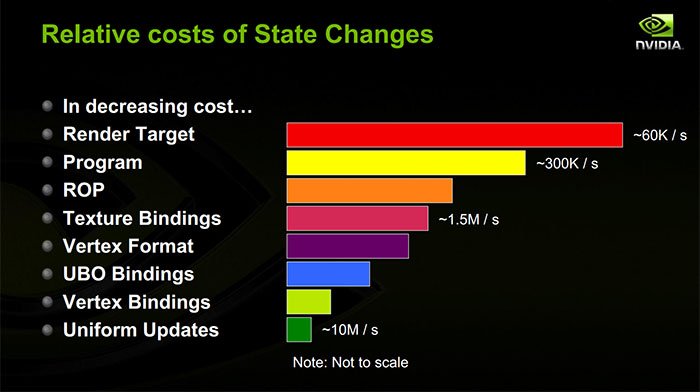
\includegraphics[width=0.6\linewidth]{assets/statecosts}
	\captionof{figure}{Costo de cambios de estado en OpenGL. Se muestra el costo de las distintas operacioens en orden inverso de cantidad de operaciones realizables por segundo para la tarjeta Nvidia GTX 480. \cite{nvidia}}
	\label{img:statechangescost}
\end{minipage}

	\begin{enumerate}
		\item El shader de vértices es simplemente \textit{passthough} lo que significa que conecta las entradas provistas por la CPU con su salida.
		\item El shader de geometría genera cinco primitivas donde cada una estará en las coordenadas correspondientes a los volúmenes de vista de las caras del hemicubo además de añadir un plano adicional de corte del dibujo necesario debido a la imposibilidad de que las caras laterales posean una resolución menor a la cara superior.
		\item El shader de fragmentos corrige el identificador local \verb|gl_PrimitiveId| a un identificador global a partir de variables uniformes que conservan el valor de caras cúbicas y triangulares que componen el objeto. Luego, escribirá el identificador de la cara detectada en la textura que le corresponda según el valor asignado por el \textit{geometry shader}.
	\end{enumerate}
	\begin{algorithm}

	\caption{Algoritmo de proyección de la escena en un hemi-cubo}
	\label{alg:renderHemicube}
	\fontsize{8}{8}\selectfont
	\begin{algorithmic}
		\Function{$computarFF$}{}
		\State $inicializarHemicubo()$ //inicializar los píxeles en 0
		\Loop{$parche \in escena$}
		\State $alinearCamara(parche)$ //alinear la cámara a la normal del parche
		\State $dibujar(escena)$ //dibujar la escena en el hemi-cubo (GPU)
		\State $hemicubo \gets leerHemicubo()$ //leer los píxeles del hemi-cubo
		\State $procesarHemicubo(parche, hemicubo)$ //hallar la fila asociada al parche
		\EndLoop
		\EndFunction
	\end{algorithmic}
\end{algorithm}

	\item En última instancia es necesario procesar la información del hemi-cubo dibujado para obtener una nueva fila de la matriz $\mathbf{F}$. Para esto, se suman los delta factores de forma de los pixeles para cada partche de la escena. Este proceso puede ser realizado tanto en GPU como CPU y sigue el patrón que se muestra en el Algoritmo \ref{alg:processHemicube}. Ambos métodos fueron implementados y se detallan a continuación:
	\begin{itemize}
		\item Computar factores de forma en GPU: Se utilizan \textit{compute shaders} para reducir las cinco texturas que componen el hemi-cubo en un único \textit{Shader Buffer Object} que representa un arreglo de bytes en la GPU. En este caso, el arreglo representará una fila completa de la matriz. Para calcular cada entrada se utiliza una textura inmutable (es decir, no modificable) auxiliar que contiene los valores de corrección expresados en las Eqs. \eqref{eq:ff} y \eqref{eq:ffgreenberg} en conjunción con la función \verb|atomicAdd| para sumar las componentes de los factores de forma de cada elemento. Al ser la GPU un multiprocesador puede ocurrir que varios hilos intenten sumar en la misma celda de \textbf{F} al mismo tiempo y la operación \verb|atomicAdd| obliga a realizar esas operaciones secuencialmente.
		Es posible acceder a este buffer desde la CPU mediante la función \verb|glMapBuffer|, que a través del dispositivo DMA (del inglés \textit{Direct Memory Access}) permite la lectura de la memoria VRAM (localizada físicamente en la GPU) de forma directa, aunque requiere de la sincronización entre GPU-CPU.
		No obstante, dada la naturaleza de las tarjetas gráficas el uso de estructuras de control que evalúen condiciones en tiempo de ejecución generan divergencia de hilos y por tanto reducen drásticamente el rendimiento del algoritmo.
		\item Computar factores de forma en CPU: Con el objetivo de aumentar el rendimiento del algoritmo se utiliza la reducción en CPU, en este caso, se utiliza la función \verb|glReadPixels| que sincroniza la GPU y copia el contenido de la memoria VRAM en la memoria RAM. Luego, se inician hilos de CPU que procesan la información de manera similar a la GPU, aunque de forma secuencial para eliminar la necesidad de sincronización.  Esto se realiza concurrentemente con el procesamiento de nuevos hemi-cubos en la GPU, generando un buen nivel de paralelismo entre los dispositivos.
	\end{itemize}
 \end{enumerate}

\begin{algorithm}
\caption{Procesamiento de la fila de la matriz $\mathbf{F}$ asociada al parche, a partir de la información almacenada en una textura cúbica.}
\label{alg:processHemicube}
	\fontsize{8}{8}\selectfont
\begin{algorithmic}
		\Function{$procesarHemicubo$}{$parche, hemicubo$}
			\State $fila \gets [0,...,0]$ //inicializar fila
			\Loop{$\text{ }pixel \in hemicubo:$}
				\State $factor \gets obtenerDeltaFF(pixel)$ //buscar el valor del delta ff
				\State $parcheVisto \gets obtenerIdParche(pixel)$ //computar identificador del parche
				\If{$esValido(parcheVisto)$}
					\State $fila[parcheVisto] \gets + factor$ //añadir la fracción de ff
				\EndIf
			\EndLoop
			\State $F[parche] \gets  fila$
		\EndFunction
\end{algorithmic}
\end{algorithm}

\subsection{El algoritmo del hemisferio}
El algoritmo del hemisferio (Sección 2.2.2) fue implementado utilizando la biblioteca de traza de rayos Embree que implica una solución alternativa al método del hemi-cubo. Esta biblioteca soporta el trazado de rayos en la CPU en múltiples superficies, en particular, triángulos y cuadriláteros utilizando BHV (del inglés \textit{Bounding Volume Hirarchies}). Estas estructuras de datos se basan en árboles que sub-dividen la escena en un conjunto de volúmenes simples que encapsulan un grupo de primitivas geométricas y cada nivel garantiza la reducción de tamaño de dichas estructuras. Su utilidad radica en la simplificación del cálculo de la intersección rayo-objeto, pues el cómputo de la intersección de un rayo con un volumen envolvente tiene un costo despreciable en comparación al muestreo de todas las primitivas que están contenidas en él. La aceleración se da cuando no hay intersección entre el volumen y el rayo, en caso de "fallo" se asegura a su vez el fallo de la intersección con todas las primitivas que el volumen contiene.

\begin{algorithm}
	\caption{Cálculo de una fila de los factores de forma utilizando traza de rayos}
	\label{alg:computeff}
	\fontsize{8}{8}\selectfont
	\begin{algorithmic}
		\Function{$computarFactores$}{$face$}
			\State $fila \gets [0,...,0]$
			\State $direcciones \gets beckers(nMuestras)$ //pre-computo de las direcciones en hemisferio
			\Loop{$direccion \in direcciones:$}
			//traza de rayos desde el baricentro
			\State $interseccion \gets trazarRayo(escena, baricentro, direcciones)$ 
			\State $parcheVisto \gets obtenerIdParche(intersection)$
			\If{$esValido(parcheVisto)$}//si el id no es inválido (id del vacío)
			\State $fila[parcheVisto] \gets + \frac{1}{nMuestras}$ //añadir la fracción de ff
			\EndIf
			\EndLoop
			\State $F[parcheVisto] \gets  fila$
		\EndFunction
	\end{algorithmic}
\end{algorithm}

De forma similar al método del hemi-cubo, es necesario posicionar el origen de cada rayo a trazar en el baricentro de la superficie. Luego, recordando la Eq. \eqref{eq:ffhemiesfera}, se genera un conjunto de direcciones utilizando la distribución coseno o similar. Si bien originalmente se utilizó la generación de números aleatorios para obtener direcciones de rayos correctamente distribuidos, el uso de estos generadores perjudicó el rendimiento del algoritmo debido al grado de complejidad que tienen estos algoritmos además de resultar en la presencia de ruido en la solución final. Por esto que se decidió utilizar otro algoritmo que generan de direcciones deterministas en un hemisferio propuesto por Beckers y Beckers \cite{Beckers}. Estas direcciones son pre-calculadas y almacenadas previo al procesamiento. Esta solución puede considerarse como un muestreo determinista que permite obtener resultados con menor ruido, además de mejorar el desempeño computacional del sistema.

Luego se procede a la traza de rayos. $\mathbf{F}_{ij}$ se calculará como $\frac{nIntersecciones_{ij}}{nMuestras}$, esto significa que por cada rayo que parta de la superficie $S_{i}$ impactando $S_{j}$ se adiciona $\frac{1}{nMuestras}$ al valor de la entrada correspondiente en $\mathbf{F}$.

El muestreo de puntos partiendo del origen del hemisferio en las direcciones determinadas se calcula utilizando la función \verb|rtcIntersect1| de la biblioteca Embree, que retorna, de forma similar a OpenGL, un identificador de primitiva relativo al objeto que se intersecta. Para transformarlo en un identificador global se utilizan los valores obtenidos \verb|geomID| y \verb|primID| además de un mapa de \textit{offsets} que contienen un número con la cantidad de primitivas que anteceden a un objeto. Obtenido el conjunto de primitivas vistas, resta reducirla para generar una fila de la matriz adicionando $\frac{1}{nMuestras}$ para cada rayo.

Para manejar los distintos hilos de ejecución se utilizó una combinación entre la biblioteca estándar \verb|std::threading| y OpenMP. La primera se utilizó en combinación con \verb|std::lock| para manejar los distintos hilos de la interfaz de usuario y el procesamiento de hemisferios. Mientras que por otro lado para manejar la traza de rayo se utilizó la extensión provista por OpenMP para paralelizar ciclos \verb|for|, por lo que cada rayo se maneja en un hilo independiente de forma transparente.

\section{Cálculo de factores de forma de la componente especular}

El cálculo de factores de forma extendidos fue implementado en dos variantes para el método del hemicubo. La primera de ellas utiliza la técnica de rasterización para dibujar los rebotes especulares, mientras que la otra utiliza el trazado de rayos. Además, se implementó la extensión para el método del hemisferio utilizando trazado de rayos.

\subsection{Extensión del método del hemicubo}
Ambas variantes son métodos de “dos pasadas” donde se dibuja el hemicubo normalmente, y luego de determinar cuáles de las caras visibles tienen componente especular, se proyecta nuevamente la escena para determinar qué parches son visibles a través de la reflexión.

Los métodos utilizados son heurísticos pues se basan en aproximaciones a la reflexión para aprovechar el hardware al máximo. Hay un factor de error que depende drásticamente del área de los parches y de la disposición general de la geometría, ya que al contrario de la técnica de trazado de rayos, se conoce qué parches son visibles pero se desconoce el punto exacto del espacio que es el correspondiente a cada pixel del hemi-cubo ya que solamente se almacenan los identificadores de los parches. A su vez, con motivo de simplificar el algoritmo no se considerara el delta factor de forma en el calculo de la componente especular.

La primer variante utiliza el método de dibujado de portales en la GPU, mientras que la segunda fue implementada utilizando \textit{trazado de rayos} en la CPU.

\subsubsection{Dibujado de portales}

El dibujado de portales es una técnica que emplea la rasterización para recortar el \textit{frame buffer} en cierta área arbitraria. Particularmente, estos puntos son aquellos cubiertos por un polígono que llamaremos portal. Este portal será ubicado en el entorno tridimensional, su comportamiento emulará aquel de una ventana o una puerta. Normalmente se utiliza esta técnica para optimizar el dibujado de escenas donde la oclusión entre objetos es alta. También se utiliza en la simulación de espejos planos.

Este método puede ser realizado de forma sencilla utilizando la GPU debido a los \verb|Stencil Buffers|, que son similares a los \textit{buffers} de profundidad, pero almacenan información que indique el programador. El programador almacenará cierta información en este buffer, que será utilizada para decidir qué \textit{fragmentos} pasan la prueba del \verb|Stencil Test|. Esta prueba es una función booleana que decidirá si un elemento será dibujado o no. En este caso, los elementos que se encuentren fuera del portal fallarán la prueba.

En la implementación propuesta, el primer paso consiste en dibujar un parche cuyo coeficiente de reflexión especular es mayor a cero, como se aprecia en la Figura \ref{img:espejo}. La imagen resultante se almacenará en un \textit{stencil buffer}, como se nota en el Algoritmo \ref{alg:9}. Luego, manteniendo el mismo volumen de vista, se dibujarán los identificadores de los parches de forma similar al dibujado del hemicubo, salvo que en una textura bidimensional y utilizando el stencil buffer anteriormente mencionado. Es necesario además establecer un plano de corte en la superficie especular, con el objetivo de truncar el volúmen de vista para evitar el dibujado de los objetos que se encuentren detrás del espejo. Este proceso se realiza a una menor resolución, con el objetivo de mejorar el rendimiento y minimizar el costo de transferencia de memoria.

\begin{figure}[htbp!]
	\centering
	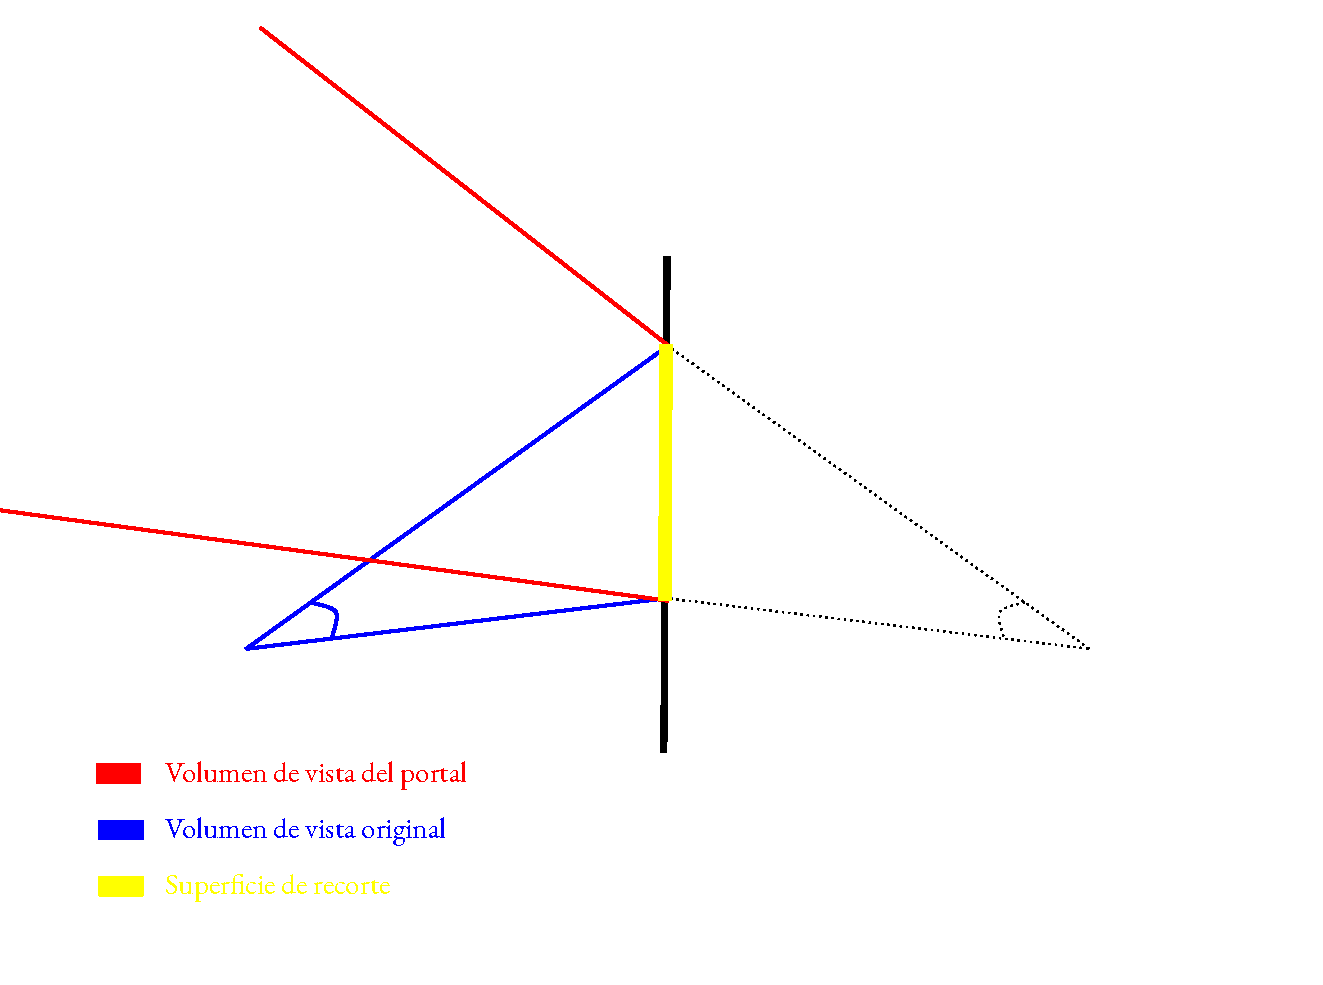
\includegraphics[width=.9\linewidth]{assets/Espejo}
	\captionof{figure}{Generación del volumen de vista para un espejo. El volúmen de vista refiere a uno de los planos del hemi-cubo.}
	\label{img:espejo}
\end{figure}

Finalmente, se obtienen los identificadores de las caras reflejadas. En caso de que existan caras reflejadas que también tengan un componente especular, se vuelven a procesar. Este procesamiento recursivo ocurre un número finito de veces, porque en este proyecto se dibujan caminos de hasta 10 rebotes. En caso de no existir superficies especulares en la imagen se utilizarán los identificadores obtenidos para distribuir el factor de forma correspondiente al fragmento del hemicubo entre los parches visualizados.

\begin{algorithm}
	\caption{Cálculo de las caras vistas utilizando dibujado de portales}
	\label{alg:9}
		\fontsize{8}{8}\selectfont
	\begin{algorithmic}
		\Function{$dibujarPortal$}{$parche, parcheObj$}
		\State $origen \gets parche.obtenerBaricentro()$
		\State $direccion \gets parche.obtenerNormal()$
		\State $configurarCamara(origen, direccion)$
		\State $seleccionarVertices(parcheObj)$
		\State $dibujarStencil()$ // dibujar área que se recortará
		\State $refDir \gets reflejar(direccion, parcheObj.obtenerNormal())$
		\State $refOrig \gets simetrico(origen, parcheObj.obtenerPlano())$
		\State $configurarCamara(refOrig, refDir)$
		\State $seleccionarVertices(escena)$
		\State $dibujar(escena)$
		\State $parchesVistos \gets leerBuffer()$
		\Loop{$parcheRef \in parchesVistos$}
		\If{$esValido(parcheRef)$}
		\State $fila[parcheRef] \gets +(\frac{1}{nSamples})$
		\If{$esEspecular(parcheRef)$} // si el coeficiente de reflexión especular es no nulo
		\State $dibujarPortal(parcheObj, parcheRef)$
		\EndIf
		\EndIf
		\EndLoop
		\EndFunction
	\end{algorithmic}
\end{algorithm}
\subsubsection{Método híbrido}

El método híbrido consiste en la utilización del trazado de rayos para computar qué parches son visualizados desde el hemicubo a través de parches especulares. Es decir, en lugar de la rasterización se utiliza la técnica de traza de rayos para calcular únicamente los caminos de reflexión especular que toma cada rayo que parte del hemicubo. Para ello, se trazarán rayos desde un conjunto de puntos pertenecientes al parche especular de manera uniformemente distribuida. La dirección es la que corresponde a la del volumen de vista, es decir, la que está dada por la diferencia entre los baricentros del parche de origen y puntos aleatorios en una grilla uniforme en el distribuidos en el parche especular. Las caras vistas, de tener componentes difusas, son las que aportarán fracciones de valor al factor de forma.

\begin{figure}[htbp!]
	\centering
	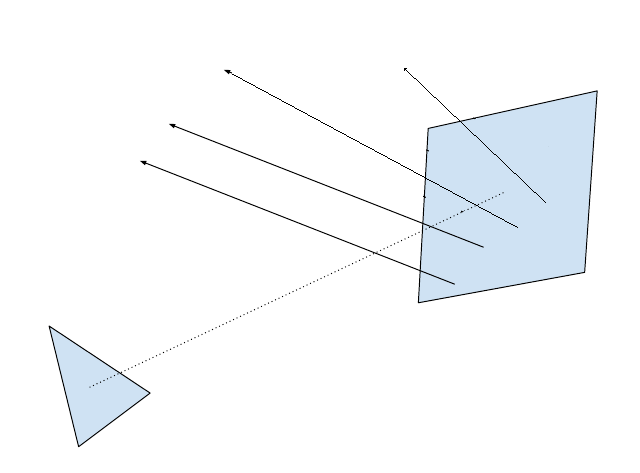
\includegraphics[width=.8\linewidth]{assets/nose}
	\captionof{figure}{Visualización del rebote de rayos al impactar en parches especulares}
	\label{img:hibrido}
\end{figure}

Esto emula el fenómeno de la reflexión, aunque introduce errores al aproximar la dirección real de reflexión. Esto se debe a que no se han de considerar las posibles oclusiones parciales entre las caras, dado que no se trazan rayos hacia el espejo en la dirección de los pixeles visibles en el hemi-cubo, sino que se eligen puntos al azar.

\begin{algorithm}
	\caption{Cálculo de las caras vistas utilizando trazado de rayos}
	\label{alg:reflections}
	\fontsize{8}{8}\selectfont
	\begin{algorithmic}
		\Function{$dibujarReflexiones$}{$parche, parcheObj$}
			\State $origenes \gets puntosEnGrilla(parcheObj)$
			\Loop{$ origen \in origenes$}
				\State $dir \gets normalizar(parche.baricentro() - parcheObj.baricentro())$
				\State $refDir \gets reflejar(dir, parcheObj.obtenerNormal())$
				\State $parche \gets trazarRayo(origen, refDir)$
				\If{$esValido(interseccion)$}
				\State $fila[parche] \gets +(\frac{1}{nMuestras})$
					\If{$esEspecular(interseccion)$}
						\State $dibujarReflexiones(parcheObj, interseccion)$
					\EndIf
				\EndIf
			\EndLoop
		\EndFunction
	\end{algorithmic}
\end{algorithm}

\subsection{Extensión del método del hemisferio}

En el caso del trazado de rayos, la extensión de los factores de forma es prácticamente trivial. Comprende la extensión de la función \verb|traceRay()|, que en lugar de retornar un único valor para la cara vista, retornará un conjunto de pares de identificadores de caras y fracción de factor de forma. Básicamente, si el rayo inicial interseca una cara cuyo coeficiente de reflexión especular es mayor a cero se almacenará el total de $k(1 - \rho^{(s)}_{j})$ (donde $k = \frac{1}{nMuestras}$) como contribuyente del factor de forma $\mathbf{F}_{ij}$ y se calcularán las siguientes intersecciones con el \textit{residuo} de la reflexión que se distribuirá entre los parches reflejados. Es decir, suponiendo que un rayo impacta $S_{k}$ desde el camino $(S_{i}, S_{j})$ donde $\rho^{(s))}_{j} \ge 0$ se agregará $k\rho^{(s))}_{j}(1 - \rho_{k})$ y se procederá de forma recursiva hasta que $\rho_{z} = 0$ para una superficie intersecada $S_{z}$ o se alcance el máximo límite de recursión cómo se aprecia en la Figura \ref{img:caminoespecular}.

\section{Cálculo de la radiosidad}

Recordando la Sección \ref{sec:vrad}, se han propuesto dos métodos para resolver el sistema, y calcular la radiosidad $\mathbf{B}$. El método "exacto" supone la resolución del sistema de ecuaciones dado por $(\mathbf{(I - RF)B} = E$, mientras que el segundo método está regido por el esquema iterativo dado por la Eq. \eqref{eq:iterativo}.

En el primer caso, debido a que las características de algunas escenas de prueba utilizadas muestran que las matrices de factores de forma pueden ser dispersas (es decir, una gran cantidad de entradas de la matriz son nulas) la implementación se realizó utilizando la biblioteca de álgebra lineal \textit{Eigen}. En este caso, dadas las características de la matriz se optó por añadir soporte para los siguientes métodos:

\begin{itemize}
	\item{De factorización}
		\begin{itemize}
			\item{Descomposición LU:} En Matrices no singulares (se ha demostrado que $\mathbf{I - RF}$ no lo es), la descomposición $\mathbf{LU}$ genera dos matrices tal que $\mathbf{I - RF} = \mathbf{M} = \mathbf{LU}$ con $\mathbf{L}$ triangular inferior y $\mathbf{U}$ triangular superior. Fácilmente se puede comprobar que  $\mathbf{M}^{-1} = \mathbf{U}^{-1} \mathbf{L}^{-1}$. Por tanto, $B =(\mathbf{U}^{-1} \mathbf{L}^{-1})E$. 
			\end{itemize}
	\item{Iterativos}
			\begin{itemize}
			\item Método de Jacobi:
				Dada una matriz cuyo radio espectral menor a uno, el método supone el uso de fórmulas como iteración de punto fijo. Dada la matriz $\mathbf{M} = \mathbf{D} + \mathbf{R}$ donde $\mathbf{D}$ es diagonal y $\mathbf{R}$ es la suma de las matrices $\mathbf{L}$ y $\mathbf{U}$. Se resuelve el sistema escribiéndolo de forma tal que la sucesión $x^{(k+1)} = \mathbf{D}^{-1}(r - \mathbf{R}^{(k+1)})$ converge al valor final.
		\end{itemize}
\end{itemize}

Por otro lado, se implementó el método completamente iterativo dado por la Eq. \eqref{eq:iterativo}. Este método es similar en precisión a los métodos iterativos  mencionados anteriormente pues no se calcula el valor exacto de $B$. Para su implementación se utilizó la biblioteca \textit{Eigen} para realizar la multiplicación de matrices dispersas con vectores de radiosidad, que tienen un largo fijo pues cada entrada representa el valor de la radiosidad en cada parche.

Finalmente, luego de calcular el vector de radiosidad se procede a la interpolación y ajuste de resultados. Dado que en OpenGL solo es posible agregar atributos a nivel de vértice y no a nivel de primitiva (parche o polígono), es necesario generar un vector extendido donde se replica el valor asignado por cara a cada uno de los vértices.

Este proceso puede realizarse de forma trivial, simplemente copiando valores o aplicando interpolación a nivel de geometría como el usado en el modelo de iluminación de \textit{Gouraud} \cite{Gouraud}. Este proceso implica balancear el valor de radiosidad para cada vértice asignándole el promedio del valor de radiosidad de cada cara adyacente(como se aprecia en la Figura \ref{img:interpolation}) en que se encuentre como muestra el Algoritmo \ref{alg:inter}.

\begin{algorithm}
	\caption{Algoritmo de interpolación de radiosidad para vértices}
	\label{alg:inter}
		\fontsize{8}{8}\selectfont
	\begin{algorithmic}
		\Function{$interpolar$}{$B$}
			\Loop{$\text{ } vertice \in escena$}
				\State $temp \gets 0$
				\State $parches \gets parches\text{ } donde\text{ } vertice\text{ } \in parche$
				\Loop{$\text{ } parche \in parches$}
					\State $temp \gets +B(parche)$
				\EndLoop
				\State $radiosidadVertice \gets \frac{temp}{cantidad(parches)}$
			\EndLoop
		\EndFunction
	\end{algorithmic}
\end{algorithm}

\begin{figure}[htbp!]
	\centering
	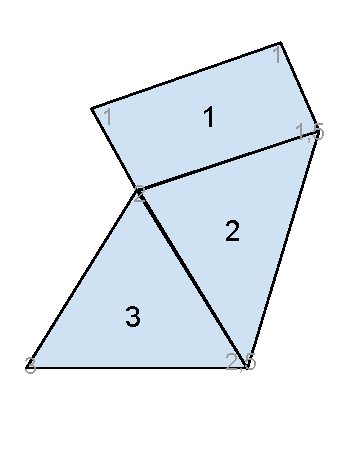
\includegraphics[width=.3\linewidth]{assets/Interpolation}
	\captionof{figure}{Ejemplificación del algoritmo de interpolación}
	\label{img:interpolation}
\end{figure}

Esta técnica genera resultados con figuras de colores menos facetados, ocultando la discretización que se realizó para aplicar el método, como se aprecia en la Figura \ref{img:interpolationres}.

\begin{figure}[htbp!]
	\centering
	\begin{subfigure}{0.7\textwidth}
		\centering
		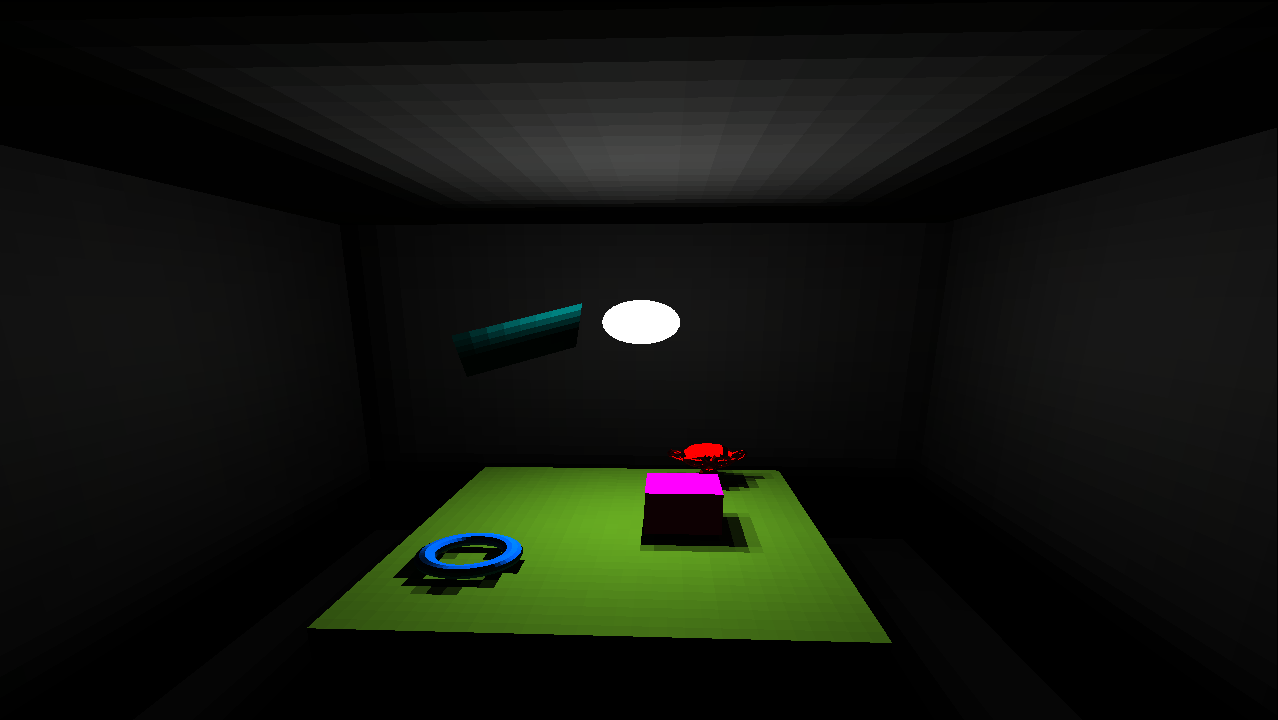
\includegraphics[width=1\linewidth]{assets/cornell-flat}
		\caption{Facetado}
	\end{subfigure}
	\begin{subfigure}{0.7\textwidth}
		\centering
		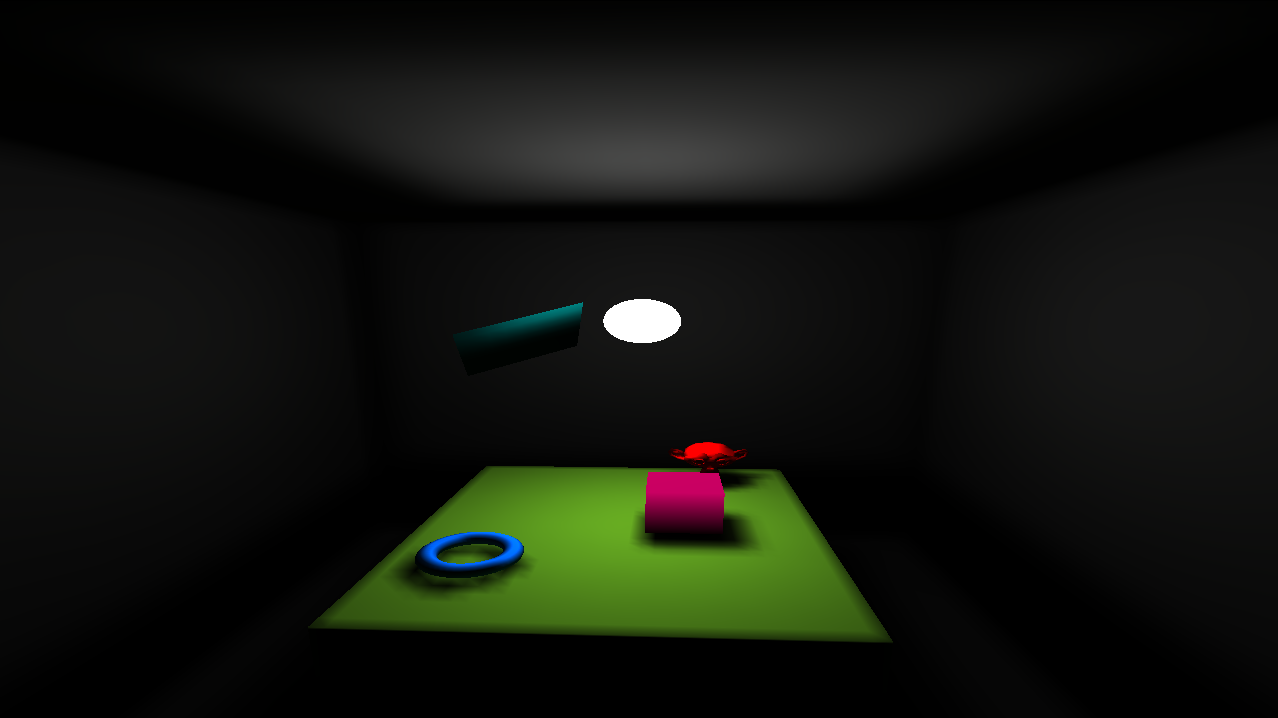
\includegraphics[width=1\linewidth]{assets/cornell-gouraud}
		\caption{Interpolación de Gouraud}
	\end{subfigure}
	\caption{Dibujado utilizando distintas funciones de interpolación}
	\label{img:interpolationres}
\end{figure}

\section {Visualización de resultados y resultados intermedios}

La visualización de resultados finales e intermedios se implementó utilizando el método de \textit{dibujado a textura en capas}. Las texturas en capas son un conjunto de imágenes de igual resolución que contienen distinta información.

El algoritmo implementado no dibuja la escena directamente en el \textit{frame buffer} global de la pantalla. Por el contrario, se dibuja en una textura auxiliar de varios niveles (cada nivel corresponde a una propiedad distinta de la escena). El primer nivel contiene la información del identificador de las caras, el segundo nivel el valor de radiosidad, el tercero el valor de emisión inicial, y el último nivel contiene los valores de los coeficientes de reflexión difusa.

Finalmente, para generar la textura que se mostrará en pantalla se utiliza un cuadrilátero unitario. Esta es una técnica estándar para proyectar un valor contenido en un buffer interno. Dependiendo de la propiedad que seleccione el usuario, se seleccionará uno de estos niveles para desplegar en pantalla.

Este método, además, añade la posibilidad de implementar la técnica de \textit{picking} que involucra el reconocimiento de la selección que realiza el usuario. Para ello, basta obtener el valor del fragmento (\verb|glReadPixels|) que se encuentra en las coordenadas del puntero dentro de la textura.

\begin{figure}[htbp!]
	\centering
		\begin{subfigure}{0.4\textwidth}
		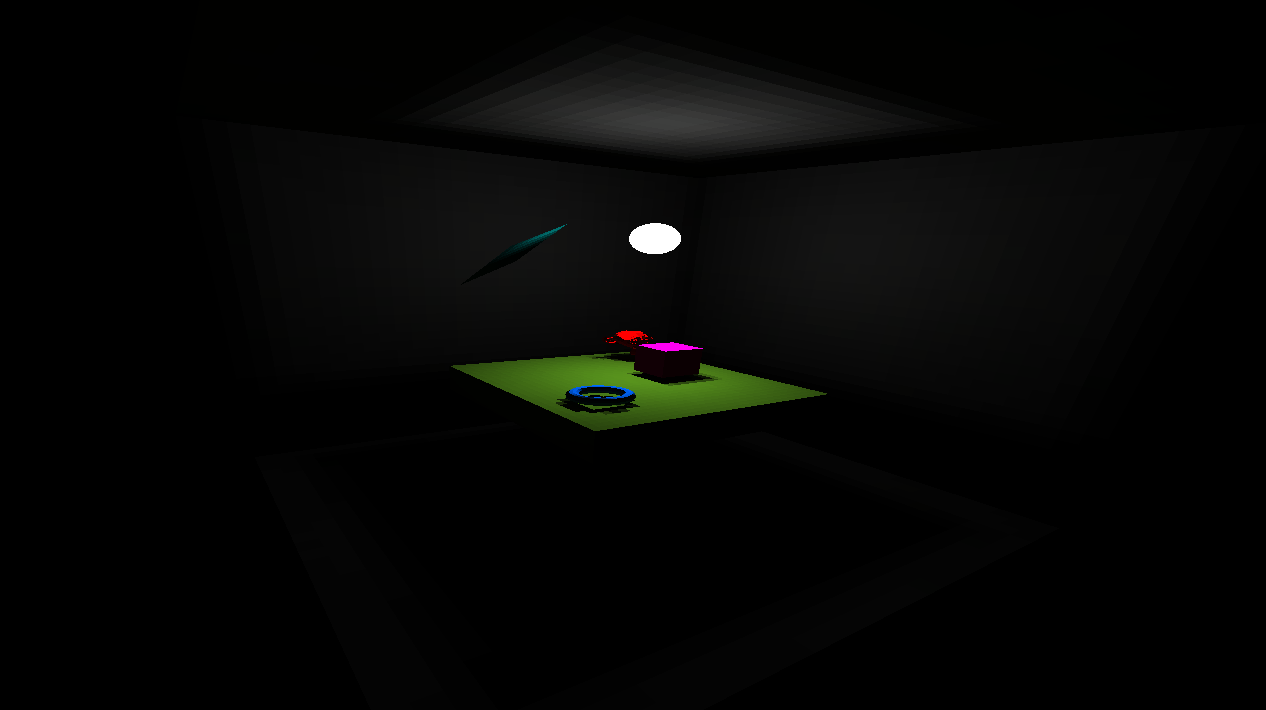
\includegraphics[width=1\linewidth]{assets/display-view(3)}
		\caption{Radiosidad sin interpolar}
	\end{subfigure}
	\begin{subfigure}{0.4\textwidth}
		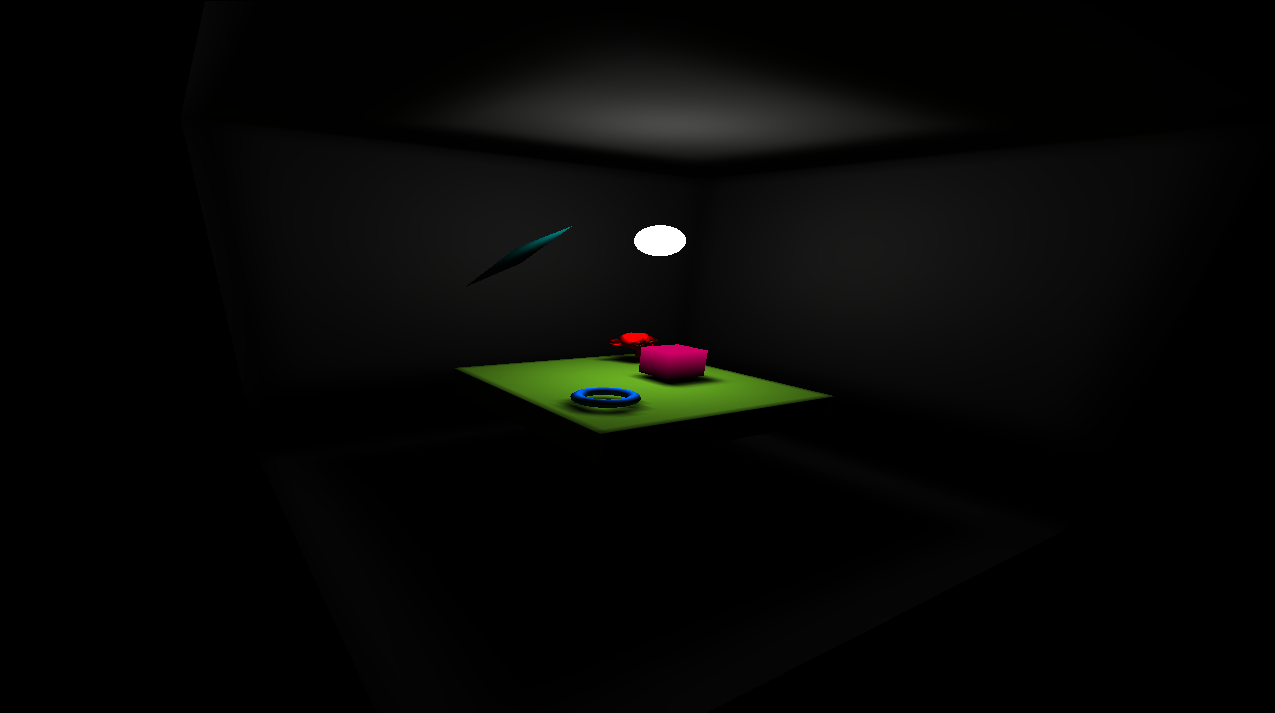
\includegraphics[width=1\linewidth]{assets/display-view(4)}
		\caption{Radiosidad interpolada}
	\end{subfigure}
	\begin{subfigure}{0.4\textwidth}
		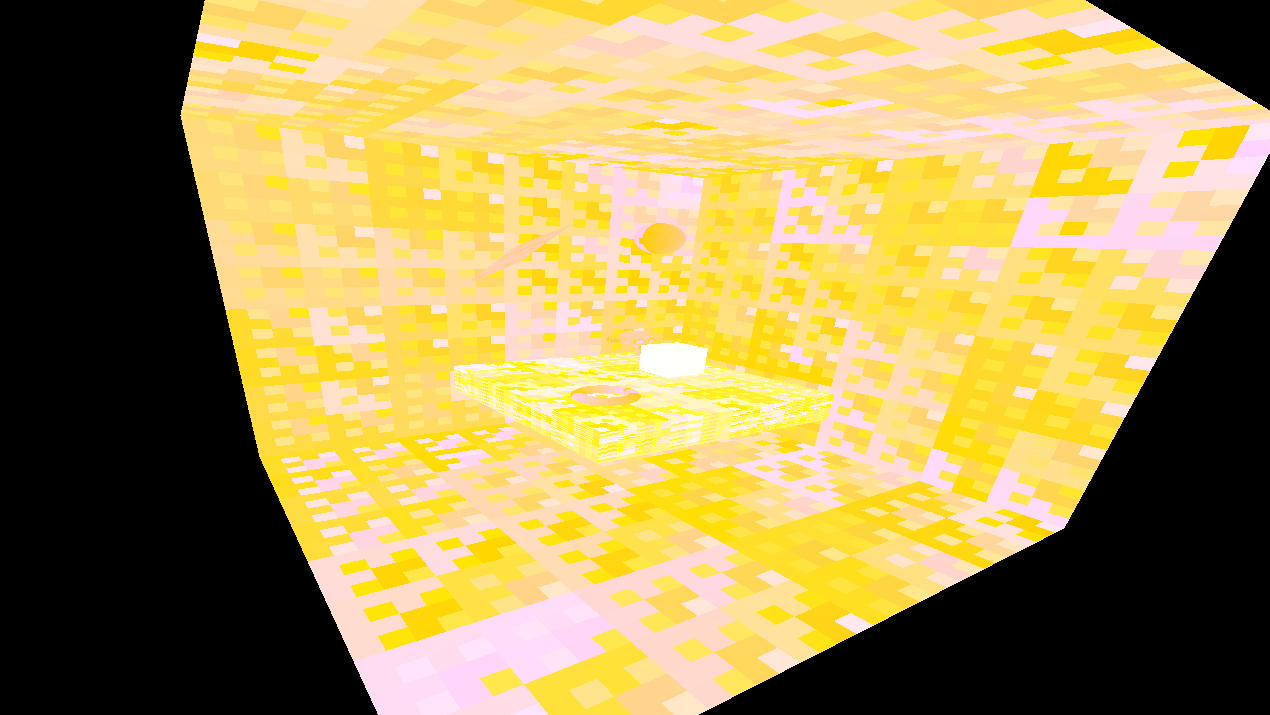
\includegraphics[width=1\linewidth]{assets/display-view(1)}
		\caption{Identificadores de parches}
	\end{subfigure}
	\begin{subfigure}{0.4\textwidth}
		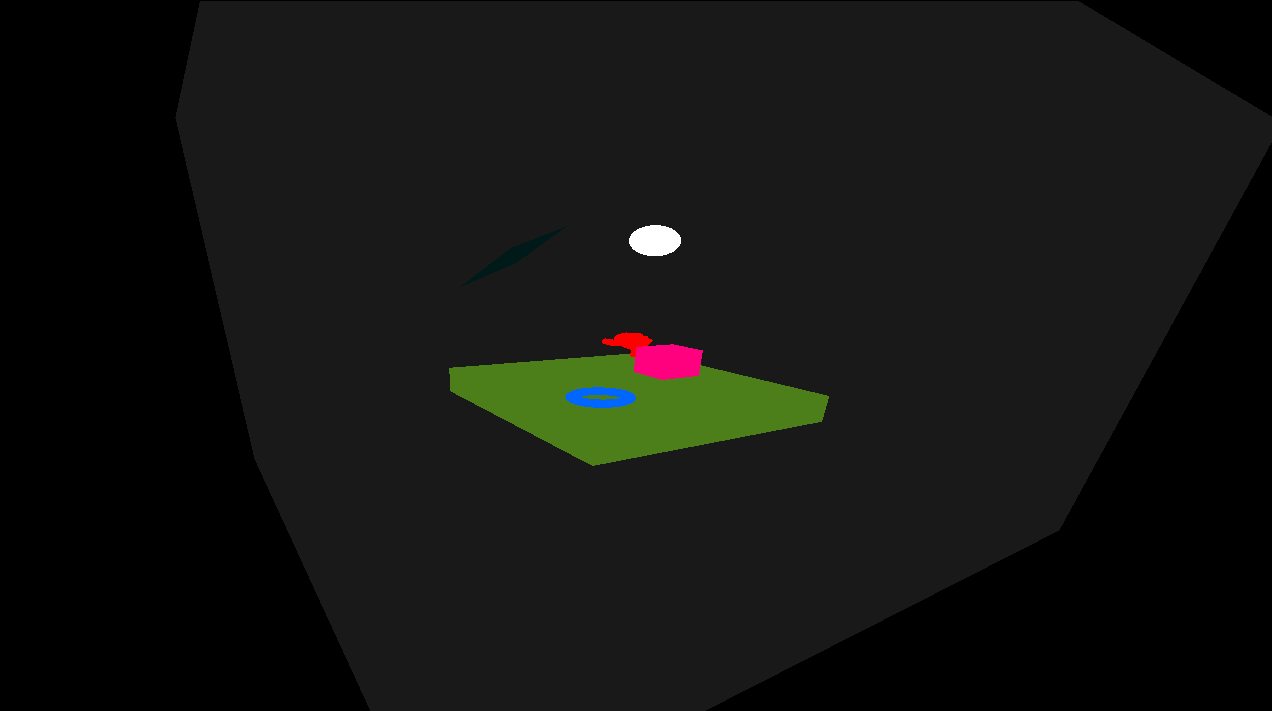
\includegraphics[width=1\linewidth]{assets/display-view(2)}
		\caption{Coeficientes de reflexión \textit{RGB}}
	\end{subfigure}
	\begin{subfigure}{0.4\textwidth}
		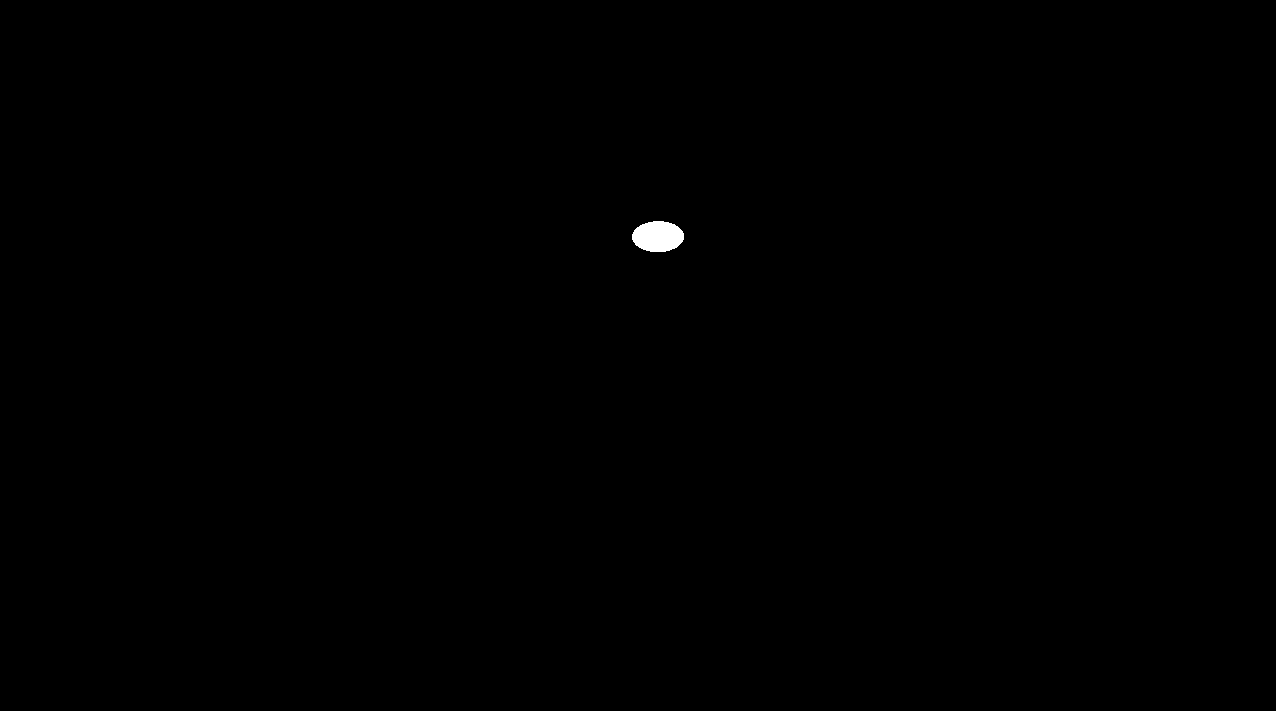
\includegraphics[width=1\linewidth]{assets/display-view(5)}
		\caption{Coeficientes de emisión}
	\end{subfigure}
	\caption{Vistas seleccionables por el usuario a través de la interfaz gráfica.}
	\label{img:displayed}
\end{figure}

\section {Interfaz de usuario}

La interfaz de usuario fue implementada utilizando la biblioteca de dibujado de interfaces gráficas en modo inmediato \textit{ImGui}. Este método de dibujado implica que los comandos de  la interfaz se ejecutan inmediatamente, de forma tal que los resultados son guardados en una máquina de estados. Los componentes dibujados dependen directamente del estado interno de la aplicación. Este método fue utilizado en versiones anteriores de OpenGL o Direct3D. Esta biblioteca implica la simplificación de la programación dada su capacidad de extenderse a diversas plataformas y por minimizar el impacto en el rendimiento de la aplicación en caso de ser utilizada.

Entre los componentes implementados que se observan en la Figura \ref{img:ui-ex} se encuentran:

\begin{itemize}
	\item Menú: El menú principal permite importar o exportar geometría (en formato Waveform OBJ utilizando un parser también implementado) y sus propiedades además de la matriz de factores de forma y editar las configuraciones del motor de dibujado.
	\item Panel de geometría: El panel de geometría permite editar el modo de seleccionado (cara, objeto) y visualizar qué cara se ha seleccionado.
	\item Panel de preprocesado: Este panel permite configurar y ejecutar las dos etapas de preprocesado (cálculo de factores de forma y radiosidad).
	\item Panel de iluminación: Permite editar características de los materiales de los objetos como los coeficientes de reflexión difusa, especular y emisión.
	\item \textit{Log}: El \textit{Log} imprime un conjunto de propiedades y detalles del proceso que pueden resultar interesantes, como por ejemplo los tiempos empleados.
\end{itemize}

\begin{figure}[htbp!]
	\centering
	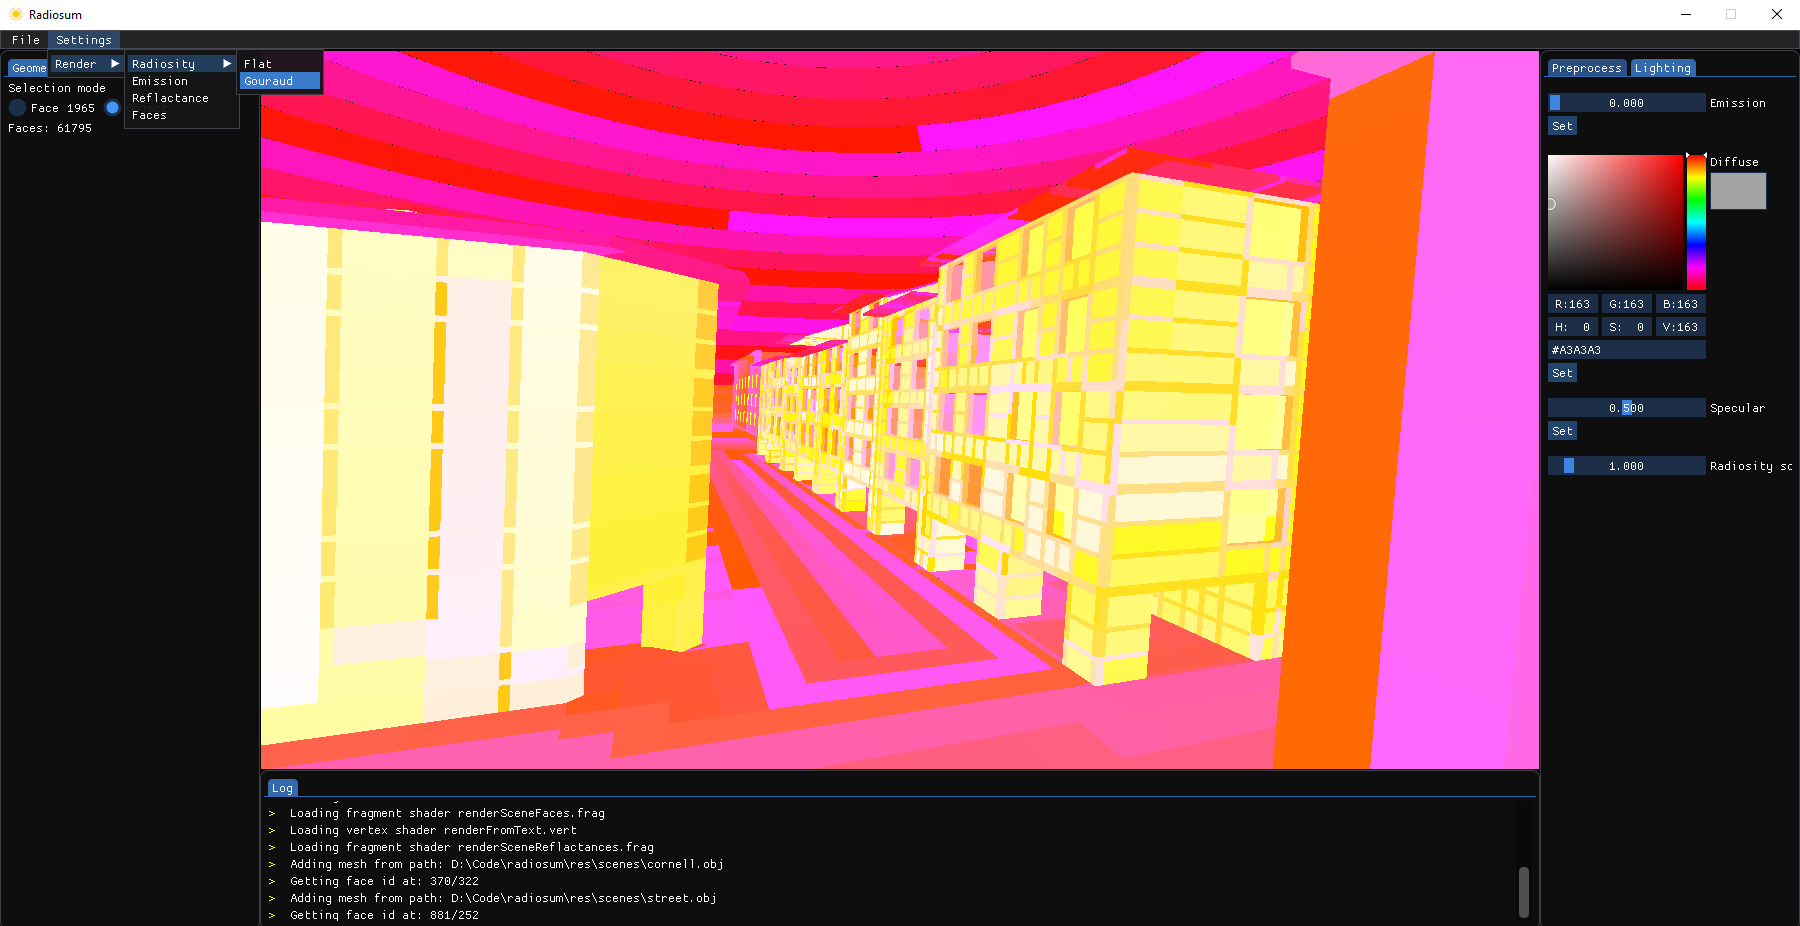
\includegraphics[width=1\linewidth]{assets/ui-ex}
	\caption{Interfaz gráfica implementada.}
	\label{img:ui-ex}
\end{figure}